% ==============================================================================
\chapter{Simulation: Full Order Model (FOM)}
\label{ch:fom}
% ==============================================================================

\section{Governing Dynamic Equations}
To simulate the dynamic response of the parameterized structure, we resolve the semi-discrete second-order system of equations of motion:
\begin{equation}
        \mat{M}(\boldsymbol{\mu}) \ddot{\underline{\mathbf{U}}}(t) + \mat{C}(\boldsymbol{\mu}) \dot{\underline{\mathbf{U}}}(t) + \mathbf{F}_{\text{int}}(\underline{\mathbf{U}}(t); \boldsymbol{\mu}) = \lambda(t) \mathbf{F}_{\text{ext}}(\boldsymbol{\mu})
\end{equation}
where:
\begin{itemize}
    \item $\mat{M}(\boldsymbol{\mu})$ is the consistent global mass matrix.
    \item $\mat{C}(\boldsymbol{\mu})$ is the viscous damping matrix.
    \item $\mathbf{F}_{\text{int}}(\underline{\mathbf{U}}(t); \boldsymbol{\mu})$ is the internal force vector, which is state-dependent under geometric nonlinearities.
    \item $\mathbf{F}_{\text{ext}}(\boldsymbol{\mu})$ is the spatial profile of the external loads, and $\lambda(t)$ is the time-dependent loading factor.
\end{itemize}

The global consistent mass matrix $\mat{M}$ is assembled element-wise using Gauss-Legendre quadrature:
\begin{equation}
        \mat{M}_{e, ab} = \int_{-1}^{1} \int_{-1}^{1} \rho R_a(\xi, \eta) R_b(\xi, \eta) |J(\xi, \eta)| \, d\xi \, d\eta
\end{equation}
where $\rho$ is the material mass density. The viscous damping matrix $\mat{C}$ is modeled using the classical Rayleigh formulation:
\begin{equation}
        \mat{C} = \alpha_M \mat{M} + \beta_K \mat{K}_0
\end{equation}
where $\alpha_M$ and $\beta_K$ are the mass-proportional and stiffness-proportional damping factors, and $\mat{K}_0$ is the baseline linear stiffness matrix.

\section{Geometric Nonlinearity Framework}
Under large displacement conditions, the infinitesimal strain assumptions are invalid. To model large deflections of the cantilever beam, we employ a geometrically nonlinear kinematic framework. The Green-Lagrange strain tensor $\mat{E}$ is defined as:
\begin{equation}
    \mat{E} = \frac{1}{2} \left( \nabla \vect{u} + \nabla \vect{u}^T + \nabla \vect{u}^T \nabla \vect{u} \right)
\end{equation}
where $\nabla \vect{u}$ represents the gradient of the continuous displacement field.

The internal force vector $\mathbf{F}_{\text{int}}(\underline{\mathbf{U}})$ is evaluated over the initial configuration $\Omega_0$ using the nonlinear strain-displacement matrix $\mat{B}_L(\underline{\mathbf{U}})$ and the Second Piola-Kirchhoff stress vector $\vect{S} = [S_{xx}, S_{yy}, S_{xy}]^T$:
\begin{equation}
        \mathbf{F}_{\text{int}}(\underline{\mathbf{U}}) = \int_{\Omega_0} \mat{B}_L^T(\underline{\mathbf{U}}) \vect{S} \, d\Omega_0
\end{equation}
The nonlinear strain-displacement matrix $\mat{B}_L(\underline{\mathbf{U}})$ is decomposed into a displacement-independent part $\mat{B}_0$ and a displacement-dependent nonlinear part $\mat{B}_{\text{NL}}(\underline{\mathbf{U}})$:
\begin{equation}
        \mat{B}_L(\underline{\mathbf{U}}) = \mat{B}_0 + \mat{B}_{\text{NL}}(\underline{\mathbf{U}})
\end{equation}

The state-dependent tangent stiffness matrix $\mat{K}_T(\underline{\mathbf{U}})$ is obtained by taking the variation of the internal force vector:
\begin{equation}
    \mat{K}_T(\underline{\mathbf{U}}) = \mat{K}_e(\underline{\mathbf{U}}) + \mat{K}_{\sigma}(\underline{\mathbf{U}}) = \left( \mat{K}_0 + \mat{K}_L(\underline{\mathbf{U}}) \right) + \mat{K}_{\sigma}(\underline{\mathbf{U}})
\end{equation}
where $\mat{K}_L(\underline{\mathbf{U}})$ is the large-displacement stiffness matrix accounting for kinematic coupling, and $\mat{K}_{\sigma}(\underline{\mathbf{U}})$ is the initial stress (geometric) stiffness matrix. The large-displacement stiffness matrix is defined as:
\begin{equation}
        \mat{K}_L(\underline{\mathbf{U}}) = \int_{\Omega_0} \left( \mat{B}_0^T \mat{D} \mat{B}_{\text{NL}}(\underline{\mathbf{U}}) + \mat{B}_{\text{NL}}^T(\underline{\mathbf{U}}) \mat{D} \mat{B}_0 + \mat{B}_{\text{NL}}^T(\underline{\mathbf{U}}) \mat{D} \mat{B}_{\text{NL}}(\underline{\mathbf{U}}) \right) \, d\Omega_0
\end{equation}
The geometric stiffness matrix is formulated as:
\begin{equation}
        \mat{K}_{\sigma}(\underline{\mathbf{U}}) = \int_{\Omega_0} \mat{G}^T \mat{M}(\vect{S}) \mat{G} \, d\Omega_0
\end{equation}
For each control point node $a$, the displacement gradient interpolation block $\mat{G}_a$ and the stress mapping block matrix $\mat{M}(\vect{S})$ are:
\begin{equation}
        \mat{G}_a = \begin{bmatrix} \frac{\partial R_a}{\partial x} & 0 \\[0.3em] \frac{\partial R_a}{\partial y} & 0 \\[0.3em] 0 & \frac{\partial R_a}{\partial x} \\[0.3em] 0 & \frac{\partial R_a}{\partial y} \end{bmatrix}, \quad \mat{M}(\vect{S}) = \begin{bmatrix} \mat{S}_{\text{mat}} & \mat{0} \\ \mat{0} & \mat{S}_{\text{mat}} \end{bmatrix}, \quad \mat{S}_{\text{mat}} = \begin{bmatrix} S_{xx} & S_{xy} \\ S_{xy} & S_{yy} \end{bmatrix}
\end{equation}

\begin{figure}[htbp]
    \centering
    \begin{tikzpicture}[
        node distance=1.6cm,
        block/.style={rectangle, draw=blue!70, fill=blue!5, thick, rounded corners, minimum width=6cm, minimum height=0.9cm, align=center, font=\sffamily\small},
        process/.style={rectangle, draw=orange!70, fill=orange!5, thick, minimum width=6cm, minimum height=0.9cm, align=center, font=\sffamily\small},
        arrow/.style={thick,->,>=stealth}
    ]
        % Left Column: Naive Physical
        \node [block] (naive_start) {Naive Physical Path \\ $\Omega(\boldsymbol{\mu})$};
        \node [process, below of=naive_start, node distance=1.6cm] (remesh) {Regenerate Mesh \\ $N(\boldsymbol{\mu})$ varies};
        \node [process, below of=remesh, node distance=1.6cm] (assemble) {Assemble Stiffness $K(\boldsymbol{\mu})$ \\ High Cost, Online};
        
        % Right Column: Mapped Reference
        \node [block, right=1.5cm of naive_start] (mapped_start) {Reference Map Path \\ $\hat{\Omega}$};
        \node [process, below of=mapped_start, node distance=1.6cm] (static_mesh) {Static Reference Mesh \\ $N$ is constant};
        \node [process, below of=static_mesh, node distance=1.6cm] (pullback) {Pullback Integrals \\ Jacobian $\mat{J}(\boldsymbol{\mu})$};
        
        % Connections
        \draw [arrow] (naive_start) -- (remesh);
        \draw [arrow] (remesh) -- (assemble);
        \draw [arrow] (mapped_start) -- (static_mesh);
        \draw [arrow] (static_mesh) -- (pullback);
    \end{tikzpicture}
    \caption{Visual workflow comparing physical-domain mesh regeneration (Naive) against static reference-configuration pullback mapping.}
    \label{fig:remesh_vs_pullback}
\end{figure}

\section{Implicit Dynamics \& Incremental Newton-Raphson Solver}
To resolve the semi-discrete second-order system of equations of motion, we couple the implicit \textbf{Newmark-$\beta$} scheme with an incremental \textbf{Newton-Raphson} solver. The dynamic tangent system is linearized and iteratively solved at each time step to trace the geometrically nonlinear deformation path. The detailed solver steps are formalized in Algorithm \ref{alg:fom_dynamics}.

\begin{algorithm}[htbp]
\caption{Full Order Model (FOM) Implicit Dynamics Solver}
\label{alg:fom_dynamics}
\begin{algorithmic}[1]
\Procedure{StepDynamicsFOM}{$\vect{U}_n, \dot{\vect{U}}_n, \ddot{\vect{U}}_n, \mu, r, \sigma, \Delta t$}
    \State Predict displacements and velocities using Newmark-$\beta$ ($\beta=0.25, \gamma=0.5$):
    \State $\vect{U}_{\text{pred}} \gets \vect{U}_n + \Delta t \dot{\vect{U}}_n + \Delta t^2 (0.5 - \beta) \ddot{\vect{U}}_n$
    \State $\dot{\vect{U}}_{\text{pred}} \gets \dot{\vect{U}}_n + \Delta t (1 - \gamma) \ddot{\vect{U}}_n$
    \State Initialize step values: $\vect{U}^{k=0} \gets \vect{U}_{\text{pred}}$, \quad $\dot{\vect{U}}^{k=0} \gets \dot{\vect{U}}_{\text{pred}}$, \quad $\ddot{\vect{U}}^{k=0} \gets \ddot{\vect{U}}_n$
    \State Assemble mass matrix $\mat{M}(\mu, r)$
    \State Compute external force vector $\vect{F}_{\text{ext}}^{n+1} \gets \text{calculateExternalForceVector}(t_{n+1})$
    \For{$k = 0, 1, \dots$ to $N_{\text{max}}$}
        \State Assemble physical or mapped tangent operators:
        \State $\mat{K}_T, \vect{F}_{\text{int}} \gets \text{assembleNonlinearForceAndStiffness}(\mu, r, \vect{U}^k)$
        \State Compute damping $\mat{C} \gets \alpha_M \mat{M} + \beta_K \mat{K}_T$
        \State Update accelerations and velocities:
        \State $\ddot{\vect{U}}^k \gets \frac{\vect{U}^k - \vect{U}_n - \Delta t \dot{\vect{U}}_n}{\beta \Delta t^2} - \frac{0.5-\beta}{\beta}\ddot{\vect{U}}_n$
        \State $\dot{\vect{U}}^k \gets \dot{\vect{U}}_{\text{pred}} + \gamma \Delta t \ddot{\vect{U}}^k$
        \State Compute dynamic residual:
        \State $\vect{R}_{\text{dyn}} \gets \vect{F}_{\text{ext}}^{n+1} - \mat{M} \ddot{\vect{U}}^k - \mat{C} \dot{\vect{U}}^k - \vect{F}_{\text{int}}$
        \State Zero out clamping boundary rows/entries in residual $\vect{R}_{\text{dyn}}$
        \If{$\|\vect{R}_{\text{dyn}}\|_2 < \epsilon_{\text{tol}}$} \textbf{break}
        \EndIf
        \State Assemble effective tangent matrix: $\mat{K}_{\text{eff}} \gets \mat{K}_T (1 + \frac{\gamma \beta_K}{\beta \Delta t}) + \mat{M} (\frac{1}{\beta \Delta t^2} + \frac{\gamma \alpha_M}{\beta \Delta t})$
        \State Apply penalty Dirichlet clamping at clamped left edge ($x=0$):
        \State $\mat{K}_{\text{eff}}[i, i] \gets 10^{30}$, \quad $\vect{R}_{\text{dyn}}[i] \gets 0$ for all boundary DOFs $i$
        \State Solve linear correction: $\Delta \vect{U} \gets \text{gaussianElimination}(\mat{K}_{\text{eff}}, \vect{R}_{\text{dyn}})$
        \State Update state: $\vect{U}^{k+1} \gets \vect{U}^k + \Delta \vect{U}$
    \EndFor
    \State Update history: $\vect{U}_{n+1} \gets \vect{U}^k, \quad \dot{\vect{U}}_{n+1} \gets \dot{\vect{U}}^k, \quad \ddot{\vect{U}}_{n+1} \gets \ddot{\vect{U}}^k$
    \State \Return $\vect{U}_{n+1}, \dot{\vect{U}}_{n+1}, \ddot{\vect{U}}_{n+1}$
\EndProcedure
\end{algorithmic}
\end{algorithm}

For higher accuracy in transient simulations, we also support the \textbf{generalized-$\alpha$ method}. This scheme extends Newmark-$\beta$ by evaluating the system at intermediate stages $\alpha_m$ and $\alpha_f$ to introduce high-frequency numerical damping while minimizing low-frequency dissipation:
\begin{equation}
    \hat{\mathbf{M}}(\boldsymbol{\mu}) \underline{\ddot{\mathbf{U}}}_{t+\alpha_m} + \mathbf{F}_{\text{int}}(\underline{\mathbf{U}}_{t+\alpha_f}; \boldsymbol{\mu}) = \lambda(t+\alpha_f) \hat{\mathbf{F}}_{ext}(\boldsymbol{\mu})
\end{equation}

\section{Quantities of Interest \& Numerical Results}
To evaluate the dynamic performance of the Full Order Model (FOM) under shape variations, we track two primary physical Quantities of Interest (QoI) over the time interval $t \in [0, 10]$ seconds:
\begin{enumerate}
    \item \textbf{Tip Vertical Deflection} $U_y(t)$: Evaluated as the spatial average of the vertical displacement component along the rightmost boundary edge ($x = L$).
    \item \textbf{Maximum Von Mises Stress} $\sigma_{\text{VM}}$: Extracted at the quadrature integration points adjacent to the symmetric top and bottom circular notches to monitor stress concentration factors.
\end{enumerate}

Under a harmonic loading force $F(t) = F_0 \sin(\omega_{\text{ext}} t)$ applied at the tip, where $F_0 = 150.0$ N and $\omega_{\text{ext}} = 1.2$ rad/s, the beam undergoes large-displacement geometrically nonlinear oscillations. The average vertical deflection peaks at approximately $8.54$ mm. Due to the throat area reduction caused by the parameter-dependent circular notches, severe stress concentrations occur near the notch boundaries, where the local Von Mises stresses reach up to $210$ MPa, compared to a baseline bending stress of under $75$ MPa in unnotched regions.

\begin{figure}[htbp]
    \centering
    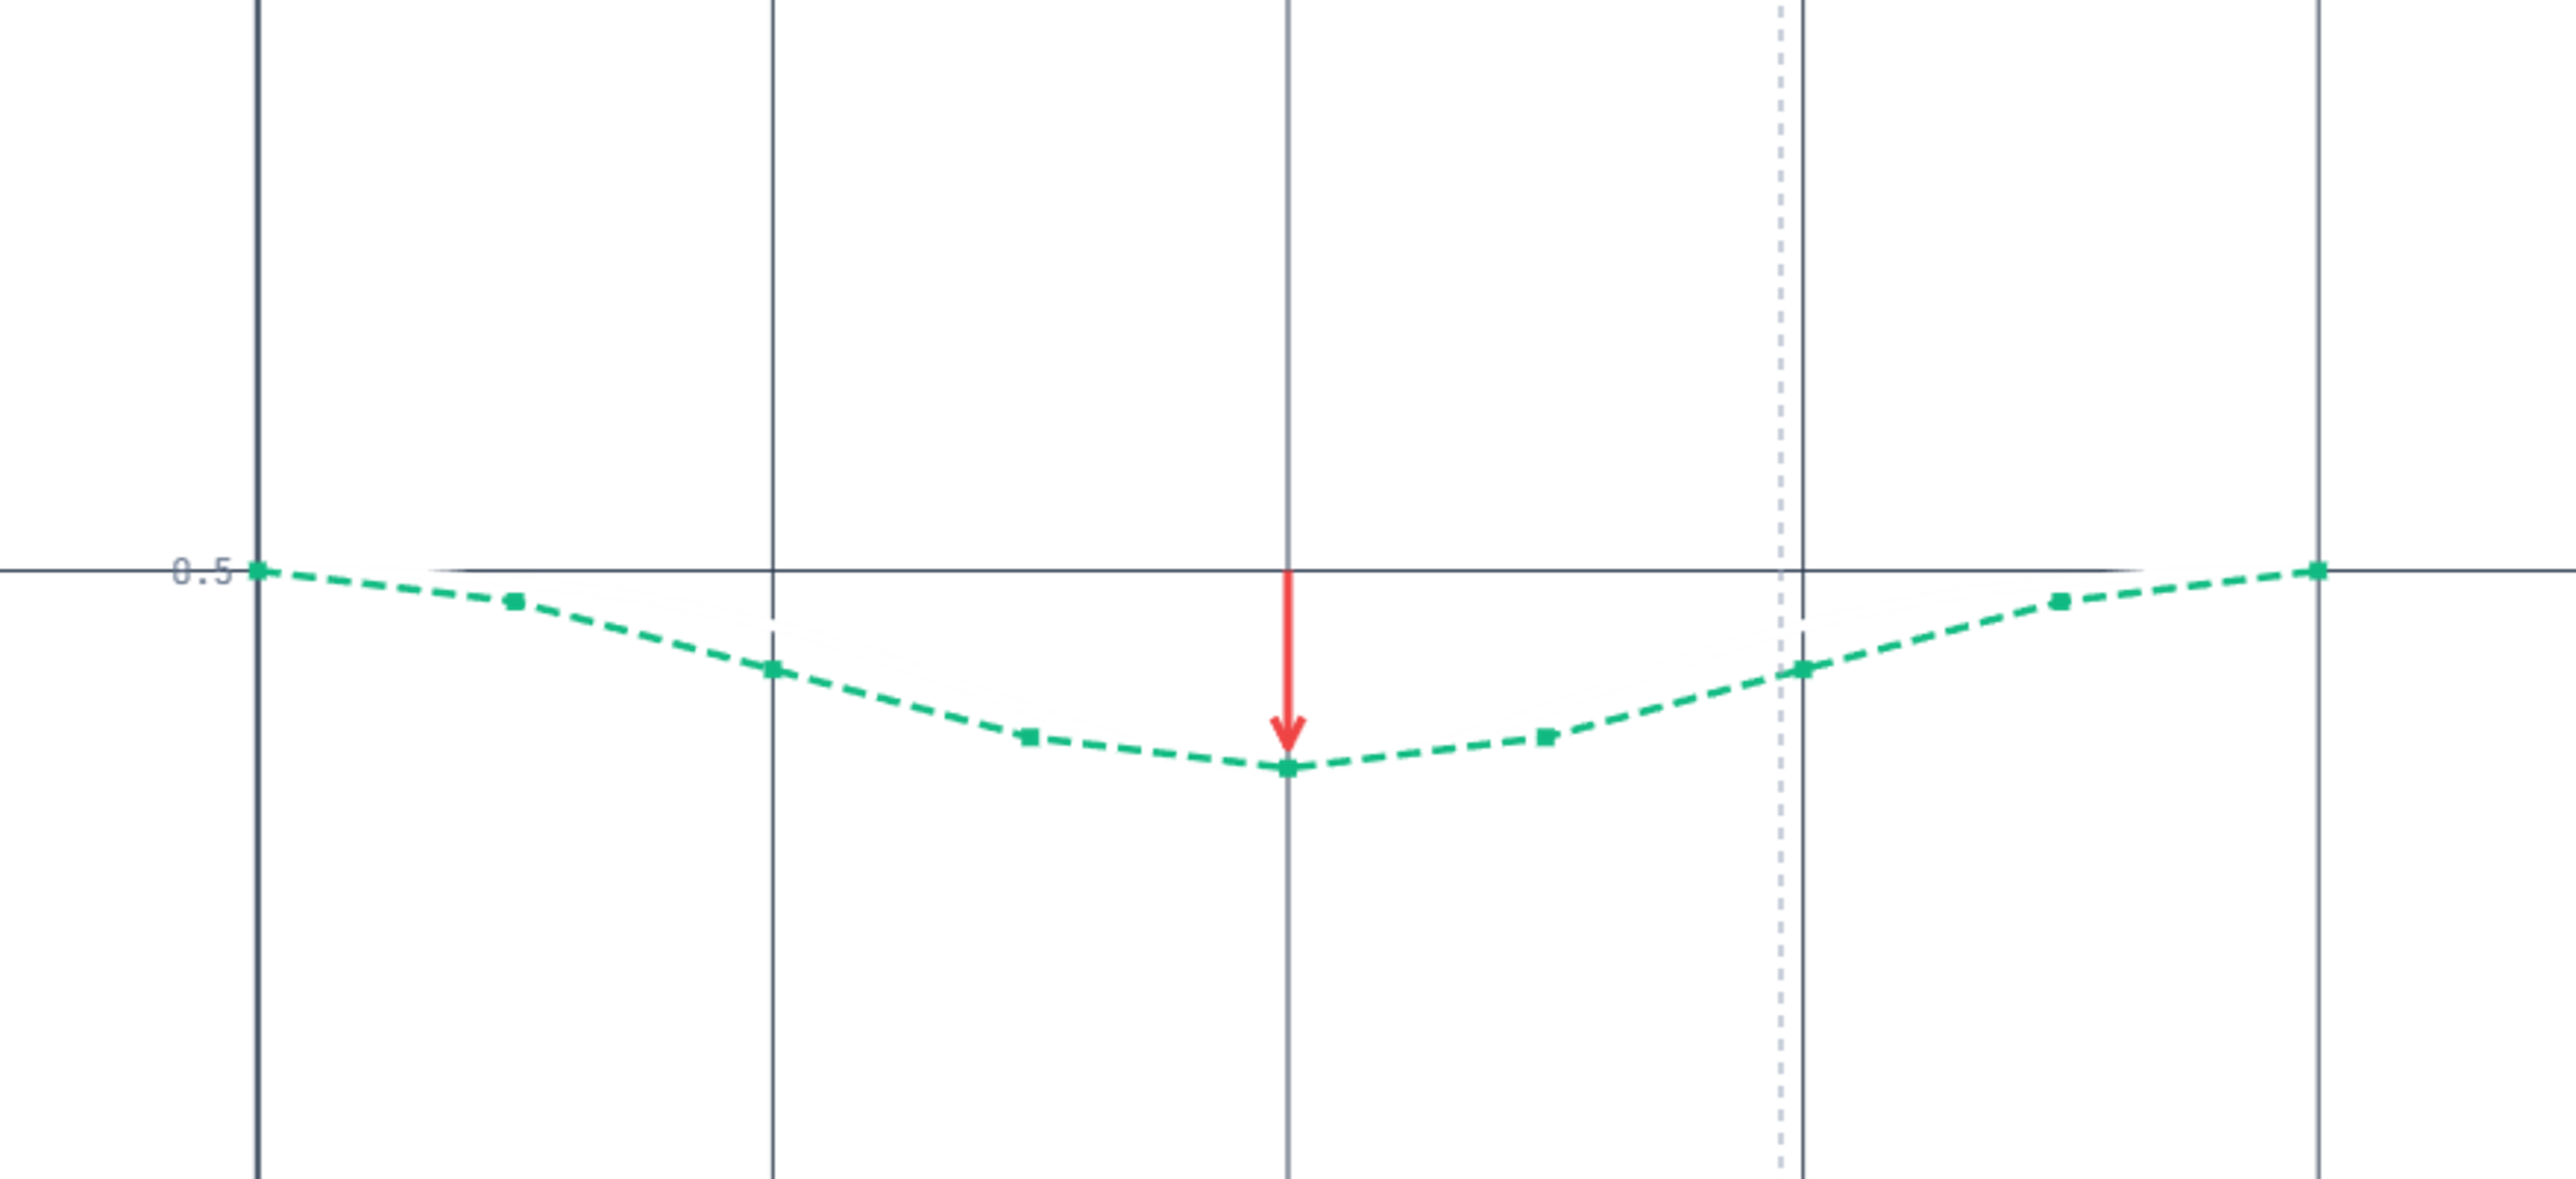
\includegraphics[width=0.8\textwidth]{chapters/4_simulation/images/iga_vs_fem_bending.png}
    \caption{Full Order Model (FOM) tip bending deflection response compared against classical high-fidelity Finite Element Method (FEM) validation baseline.}
    \label{fig:iga_vs_fem_bending}
\end{figure}

The computational costs associated with the FOM simulation are summarized as follows:
\begin{itemize}
    \item \textbf{Mesh Discretization}: $E = 3,200$ bivariate elements, corresponding to $N = 6,564$ physical degrees of freedom.
    \item \textbf{Average Assembly \& Solve Time}: Requires $142.1$ ms per time-step. Solving a complete transient window of $200$ steps requires over $28$ seconds of CPU execution.
\end{itemize}
These numerical benchmarks highlight the significant offline cost of the high-fidelity model and justify the implementation of projection-based Reduced Order Modeling in Chapter \ref{ch:rom}.


